\chapter{Projekt SmartFactory@EH-Anlage}\label{ch:data}

\section{Projekt Smart Factory-Anlage: Aufgabenstellung}\label{sec:Projekt Smart Factory-Anlage: Aufgabenstellung}

Die SmartFactory-Anlage ist eine speziell für Schulungszwecke konzipierte
Automatisierungsanlage, die von der Abteilung Expert House entwickelt wurde. Sie beinhaltet verschiedene Produkte aus dem Siemens-Produktkatalog 
wie zum Beispiel speicherprogrammierbare Steuerungen, Lichtsensoren und Motoren.
Meine Aufgabe bestand darin, zusammen mit 18 weiteren Studierenden die
Weiterentwicklung für diese Anlage durchzuführen. Dies umfasste sowohl die
vollständige Ausbesserung von und Behebung bereits bekannter Mängel, welche in einer List of Open Points (LOP) festegehalten wurden, 
als auch das Testen der Robustheit der Software. Die Software wurde nach dem 
ISA-88-Standard umgesetzt und alle Erweiterungen sollen auch nach diesem hinzugefügt werden. Zur Programmierung war 
die Siemens-Automatisierungssoftware „TIA-Portal“ zur Verwendung vorgegeben. Eine weitere Anforderung war es, die 
umfassenden Dokumentationsunterlagen in Form von Word-Dokumenten für nachfolgende Studierende auszubessern und 
gegebenenfalls mit den neuen Funktionen zu erweitern. Die Nutzung des ISA-88-Standard soll gewährleisten, das die Anlage 
ohne einen Ansprechpartner aus unserem Projektteam weiterentwickelbar ist. 


\section{Projekt Smart Factory-Anlage: Zielsetzung}\label{sec:Projekt Smart Factory-Anlage: Zielsetzung}

Das Ziel am Ende des Praxissemesters war es, die funktionsfähige
SmartFactory-Anlage weiterzuentwickeln, ihre Robustheit zu erhöhen und uns eine Grundlage für Ausbildungs- und Weiterbildungsmodule zu schaffen. 
Dafür müssen für jedes Anlagenmodul bekannte Fehler und offene Punkte aus der List of Open Points (LOP) abgearbeitet werden, sowie bei der Erkennung neuer Fehler, 
diese zur List of Open Points (LOP) hinzugefügt werden. Des Weiteren müssen die Bedingungen wie eine einheitliche HMI-Schnittstelle 
und eine leichte Bedienung der Anlage umgesetzt werden.

\section{Projekt SmartFactory-Anlage: Projektorganisation (geschrieben)}\label{sec:Projekt SmartFactory-Anlage: Projektorganisation (am ändern)}

Das Projektteam besteht aus ... Informatikstudenten und ... Elektro- und Informationstechnikstudenten sowie drei 
Fachbetreuern. Diese haben uns als ``Product Owner'' im Projekt unterstützt und geholfen.  

Das gesamte Projekt wurde auf der agilen Methode \textbf{Scrum} basierend durchgeführt. Dabei wurden jedoch Anpassungen vorgenommen, die dem 
Projektablauf und den spezifischen Umständen gerecht wurden. Wie bereits in Abschnitt~\ref{sec:Einleitung}, „Einleitung“, erläutert, wurde die 
Arbeitsphase im Expert House sowohl bei uns Informatikern als auch bei den Elektro- und Informationstechnikern durch die \textbf{SPE-Phase} 
unterbrochen, allerdings zu unterschiedlichen Zeitpunkten. Dies führte zu einem geteilten Arbeitszeitplan: In den ersten acht Wochen arbeiteten 
alle gemeinsam am Projekt, in den darauffolgenden acht Wochen nur die Elektro- und Informationstechniker, und in den abschließenden acht Wochen 
waren ausschließlich wir Informatiker beteiligt.

Trotz der Abweichungen von den klassischen Scrum-Praktiken war dieser Ansatz sinnvoll. Durch die iterative Arbeitsweise und die klare Struktur 
von Scrum konnten wir den Überblick über die aktuellen Aufgaben besser behalten. Zur Organisation der Aufgaben und Projektmeilensteine half uns 
insbesondere ein \textbf{Kanban-Board}, das die Aufgaben nach den Kategorien strukturierte. Dieses visuelle 
Hilfsmittel erleichterte die Nachverfolgbarkeit von Fortschritten erheblich und förderte die Verständlichkeit während der regelmäßigen Meetings.

Die Kombination aus Scrum-Elementen und der Verwendung des Kanban-Boards sorgte für eine verbesserte Teamkommunikation und einen reibungsloseren 
Workflow. So konnte jeder Beteiligte stets nachvollziehen, welche Aufgaben anstanden, bearbeitet wurden oder bereits abgeschlossen waren. 
Besonders in der finalen Phase, als die Teams unabhängig voneinander arbeiteten, erwies sich diese Arbeitsweise als vorteilhaft, da sie die 
Selbstorganisation förderte und klare Prioritäten setzte.

Dies führte dazu, dass an den Übergabepunkten große und kleine Änderungen klar an das andere Projektteam übergeben werden mussten.
Gleichzeitig war es essenziell, die Dokumentation stets auf dem aktuellen Stand zu halten, um eine reibungslose Weiterarbeit 
zu ermöglichen.  

Dadurch stimmten wir uns gemeinsam, Betreuer und Auszubildende, in Daily-Meetings ab. Wir arbeiteten in Zwei-Wochen-Sprints, die jeweils mit einer Vorstellung der 
Ergebnisse an die Stakeholder endeten. Diese Präsentation ist ein wichtiges Mittel um unseren Fortschritt an der Anlage zu zeigen und Punkte für die nächste 
Bearbeitung festzulegen. Eine zentrale Rolle spielte die "List of Open Points" (LOP), die zur Dokumentation 
von bestehenden Fehlern und Mängeln genutzt wurde.

Die LOP war in Dringlichkeitsstufen unterteilt:
\begin{itemize}
    \item \textbf{Sehr wichtig:} Prozessbeendende Fehler oder solche, die mechanische Schäden verursachen könnten.
    \item \textbf{Mittel:} Fehler, die den Prozess nicht vollständig stoppen, aber zu Fehlern in der Verarbeitung von Flaschen führen.
    \item \textbf{Niedrig:} Fehler mit geringeren Auswirkungen, z. B. das Herausfallen einer Kugel bei der Initialisierung der Abfüllstation.
\end{itemize}


Die Stakeholder legten diese Prioritäten fest. Für jeden Sprint suchten sich die Verantwortlichen der jeweiligen Station 
die wichtigsten Aufgaben mit der höchsten Priorität heraus und arbeiteten diese ab.  

Gerade zu bearbeitende Aufgaben und bereits abgeschlossene wurden in ein Kanban-Board eingetragen. Dies half, den Fortschritt 
zu visualisieren und machte in den Daily-Meetings deutlich, welche Aufgaben eventuell vom Plan abwichen. Dadurch konnten 
notwendige Anpassungen schnell besprochen und vorgenommen werden, um weiterhin das Projektziel in der gegebenen Zeit zu 
erreichen.  

Das Kanban-Board wurde in folgende Bereiche unterteilt:
\begin{itemize}
    \item \textbf{Aufgaben:} Hier befinden sich alle Aufgaben, die im aktuellen Sprint erledigt werden müssten, mit denen 
    sich aber noch niemand befasst hat.
    \item \textbf{In Bearbeitung:} Hier wurden die aktuell bearbeiteten Aufgaben gesammelt.
    \item \textbf{Internes Review:} Wurde eine Aufgabe abgeschlossen, wurde das Ergebnis zunächst durch einen weiteren 
    Studierenden korrekturgelesen und auf Verständlichkeit überprüft.
    \item \textbf{Ready for Review:} Eine von einem Studierenden als in Ordnung befundene Aufgabe wird noch ein weiteres 
    Mal durch einen Betreuer geprüft.
    \item \textbf{Nacharbeiten:} Wurde eine durchgeführte Aufgabe entweder von einem Betreuer oder einem Studierenden als 
    nicht in Ordnung befunden, oder es traten im Projektverlauf Probleme damit auf, ist sie in diesem Bereich zu finden.
    \item \textbf{Erledigt:} In diesem Bereich befinden sich schließlich komplett abgeschlossene Aufgaben.
\end{itemize}

Des Weiteren haben wir mit dem Siemens-Multiuser-Server gearbeitet, eine  speziell angepasste Lösung für die Zusammenarbeit an 
Automatisierungsprojekten. Das bedeutet, dass jeder Studierende eine lokale 
Instanz des Projekts hatte, diese bearbeiten und an der Anlage testen konnte. Große Änderungen konnten dann auf einen 
GIT-ähnlichen Server hochgeladen werden, von dem alle anderen Instanzen diese Änderungen wieder herunterladen konnten. 
Außerdem konnte man über ein File-Locking-System bei Dateien, an denen man gerade arbeitete, festlegen, ob ein Konflikt 
besteht, wenn zwei Studierende gleichzeitig an derselben Datei arbeiten. Dies hat ``Merge-Konflikte'' und den Verlust 
von Code verhindert, die Zusammenarbeit erleichtert und ermöglicht eine grundlegende Versionskontrolle.

\section{Projekt SmartFactory-Anlage: Projektverlauf}

\textbf{Auftaktwoche:}

Noch vor dem offiziellen Start des Projekts wurde in meiner Abteilung eine Auftaktwoche organisiert, die dazu diente, 
uns auf die bevorstehenden Aufgaben vorzubereiten. Der Schwerpunkt lag darauf, unser Wissen und unseren Umgang mit dem 
TIA Portal aufzufrischen. Obwohl wir als dual Studierende bereits einen zweiwöchigen Kurs zur Nutzung der Software 
absolviert hatten, fehlte uns durch ein Semester ohne praktische Anwendung die nötige Routine. In dieser Woche bestand 
unsere Aufgabe darin, die Steuerung eines Aufzugs mit fünf Stockwerken zu programmieren. Dabei wurden uns auch 
Programmierkonzepte wie die „State Machine“ vermittelt, die später eine wichtige Rolle bei der Entwicklung der 
SmartFactory-Anlage spielten.

\textbf{Hands-On SmartFactory-Anlage:}

Nach der Auftaktwoche wurden wir zufällig in Teams von zwei bis drei Personen eingeteilt, um die SmartFactory-Anlage 
in Betrieb zu nehmen. Ziel war es, am Ende der Woche eine Flasche, mit dem bereits bestehenden Code, vollständig durch 
die Anlage zu führen. Jedem Team wurde dabei eine spezifische Station zugewiesen. Ich war für die Abfüllstation zuständig. 
Die Aufgabenstellung war bewusst vage gehalten, um uns die Möglichkeit zu geben, die Anlage eigenständig kennenzulernen. 
Das Ergebnis bei der Abfüllstation bestand darin, das angefragte Flaschen und Deckel richtig für erstellte Aufträge 
verwendet wurden und ein Betriebsbeendender des ersten Laufbandes behoben wurden. Allerdings wurden auch einige neue Punkte, 
wie die fehlerhafte Kalibrierung des Drehtellers oder die fehlende Initalisierungsfahrt, in die LOP (List of Open Points) 
nachgetragen. Nach Abschluss dieser Aufgabe führten wir ein „Lessons Learned“ durch. Die wichtigste Erkenntnis hierbei war, 
dass die Anlage ohne einen sorgfältig erarbeiteten Plan und ein durchdachtes Konzept nicht effektiv in Betrieb 
genommen werden kann.

\textbf{Bibliotheksverantwortlicher (erweiternder Aufgabenbereich):} 

Mir wurde ein erweiterter Aufgabenbereich in Form des Bibliotheksverantwortlichen zugewiesen. Meine Aufgabe bestand darin, 
die Projektbibliothek des Multiuser-Servers konsistent zu halten. Dies ist notwendig, da Programmbausteine gemäß dem 
ISA-88-Standard, wie beispielsweise \textit{Control Modules} oder \textit{Equipment Modules}, von mehreren Instanzen im 
Projekt genutzt werden können.

Ein Lichtsensor kann beispielsweise Teil eines Förderbands oder eines Drehtellers sein. Um doppelten Code zu vermeiden und 
die Erweiterbarkeit so hoch wie möglich zu halten, wird im Code, wenn ein Lichtsensor benötigt wird, der Baustein aus der 
Projektbibliothek verwendet. Dieser Baustein wird im Projekt als neue Instanz des Bausteins aus der Projektbibliothek 
eingefügt. Möchte man den genannten Lichtsensor aktualisieren, werden alle Instanzen im Projekt sowie in der 
Projektbibliothek aktualisiert.

Da die Projektbibliothek versionsabhängig arbeitet, kann es vorkommen, dass jemand am Förderband eine Änderung vornimmt, die 
nicht mit der neuen Version des Lichtsensors kompatibel ist. Dies würde zu einem Ausfall der Lichtsensoren am Förderband 
führen. Ebenso könnte es passieren, dass auf dem Förderband noch eine ältere Version des Lichtsensors ohne die aktuellen 
Änderungen verwendet wird. Dies führt zu Inkonsistenzen, die von mir bereinigt werden mussten.

\textbf{Flaschenmanagment in der Unit:}      
wie es war -> wie es werden soll (z.b. auftrag abarbeiten wenn keine weitere flasche kommt oder ersten drei flaschen für neuen auftrag verwendet)
leerfahren in der unit (bei unbekannten Flaschen)
current order abbrechen 

\begin{figure}[h!]
    \centering
    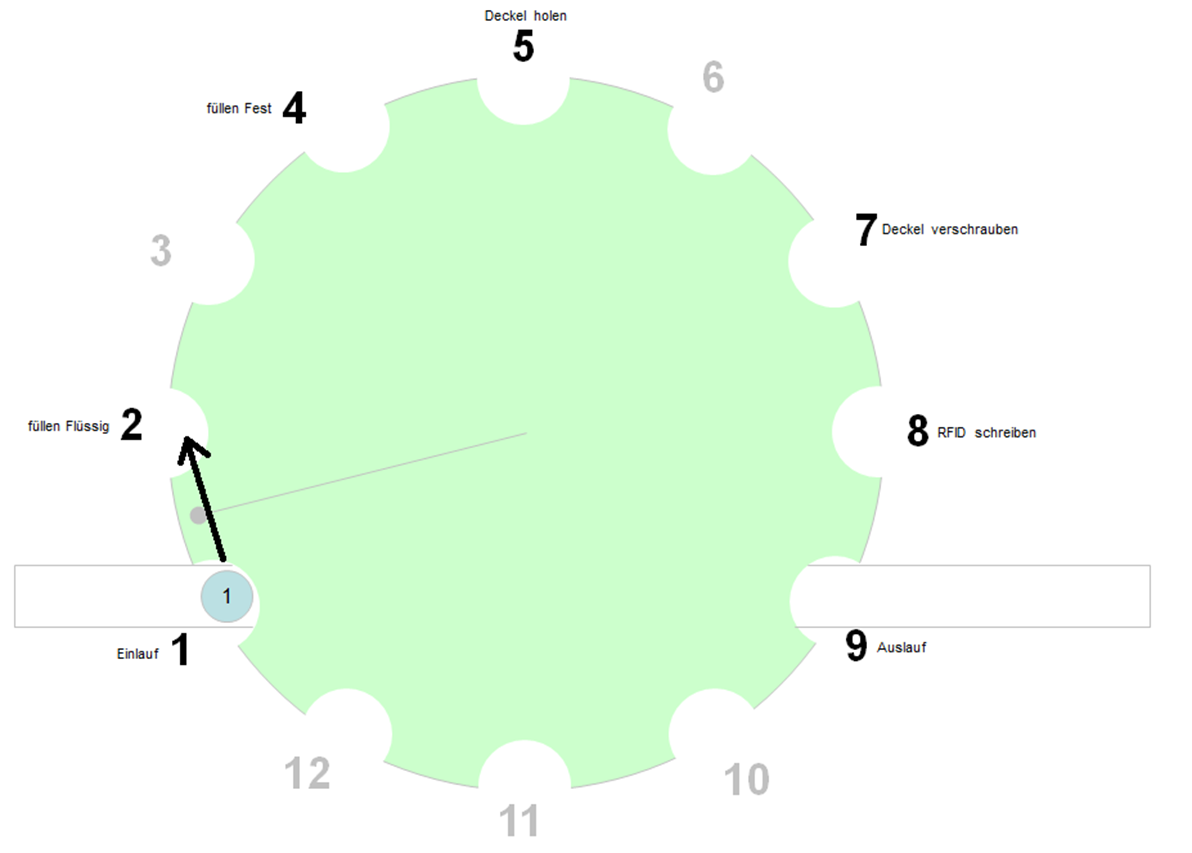
\includegraphics{figures/image.png}
    \caption{Drehteller der Abfüllanlage\cite{siemens2022}} % "Abbildung 2" wird automatisch eingefügt.
    \label{Drehteller} % Für spätere Verweise im Text.
\end{figure}

Das Flaschenmanagement der Abfüllstation wurde so umgesetzt, dass für jeden angeforderten Auftrag die benötigte Anzahl an Flaschen vom modularen 
Produktionssystem bereitgestellt wird. Diese Flaschen werden anschließend befüllt und mit Deckeln verschlossen. Ein Problem trat jedoch auf, wenn 
nicht genügend Flaschen nachgeliefert wurden. Beispielsweise konnten von 12 angeforderten Flaschen nur 9 ankommen, wodurch die Abfüllung anhielt 
und auf die Ankunft einer neuen Flasche an Position 1 des Drehtellers wartete (siehe Abbildung \ref{Drehteller}).

Um den Arbeitsfluss kontinuierlich aufrechtzuerhalten, wurde in Absprache mit den Betreuern eine Anpassung in der Unit der Abfüllstation 
vorgenommen. Diese Änderung sorgt dafür, dass, falls innerhalb von sieben Sekunden keine neue Flasche geliefert wird, die verbliebenen Flaschen, 
die sich bereits im Drehteller befinden und einem Auftrag zugewiesen wurden, dennoch abgefüllt und verschlossen werden. Dies gewährleistet eine 
höhere Effizienz und verhindert lange Stillstandszeiten der Abfüllstation.

Ein weiteres Problem betraf die Speicherung der Auftragsdaten. Diese wurden ursprünglich nicht remanent gespeichert, also nicht über einen 
PLC-Stop hinaus erhalten. Dies führte dazu, dass nach jedem Neustart oder Kaltstart der Steuerung alle Flaschen aus dem Drehteller entfernt 
werden mussten, bevor ein neuer Auftrag angelegt werden konnte. Dieses Verhalten widersprach dem Ziel, die Anlage auch für unerfahrene Bediener 
einfach und benutzerfreundlich zu gestalten.

Der Drehteller erkannte nach einem Neustart weiterhin, dass sich Flaschen an den einzelnen Positionen (1–9) befanden. Dies führte dazu, dass der 
Drehteller in einen ungültigen Zustand geriet, da er für jede Position, an der eine Aufgabe auszuführen war, fehlerhafte Zustandsinformationen 
erhielt. Beispielsweise müssen an Position 4 die Flaschen befüllt, an Position 5 die Deckel angefordert, an Position 7 die Deckel verschraubt 
und an Position 8 die RFID-Tags beschrieben werden. Ohne korrekte Zustandsinformationen konnte der Drehteller diese Aufgaben nicht ausführen, 
was die gesamte Anlage blockierte. Nach der vorgenommenen Änderung wird der Drehteller darauf hingewiesen, dass sich unbekannte Flaschen, also 
Flaschen ohne Auftrag, im Drehteller befinden. Diese Flaschen werden nun automatisch aus dem Drehteller entfernt und an das Quality Gate 
weitergeleitet.

\textbf{Drehteller:} 
fehlerfindung der knöpe -> Initalisierungsfahrt 

\textbf{Kommunikation:} 
zyklisch und unitlogik zwischen mps und Abfüllung (mit mps counter auf abfüll seite/ Einführung deckel auf flasche im udt des ordermanagments)
zwischen abfüllung und quality gate 
MODI Erklären? (hand .../ composit ...)


%/////////////////////////////////////////////////////////////////////////////////////////////////////
\section{Projekt SmartFactory-Anlage: Ergebnis}

Der finale Funktionsumfang des Projekts ist zum Zeitpunkt der Erstellung dieses Berichts noch nicht vollständig absehbar. Dennoch wurden bereits 
wesentliche Meilensteine gemäß den Vorgaben erreicht. Mit Ausnahme einiger kleinerer Bugs konnten alle kritischen, den Prozess unterbrechenden 
Fehler an der Abfüllstation behoben werden. Dadurch wurde das Hauptziel, die Robustheit der Anlage zu steigern, erfolgreich erreicht. Die 
weiteren Arbeiten konzentrieren sich nun auf die Verbesserung der Benutzerfreundlichkeit und der Erweiterbarkeit der Anlage.

Aus den täglichen Meetings und dem Feedback der Projektmitglieder geht hervor, dass auch an den anderen Stationen der Anlage deutliche 
Fortschritte erzielt wurden. Falls der Projektfortschritt bis zum Ende des Praxissemesters nicht vollständig den gesetzten Zielen entspricht, 
bieten die sorgfältig erstellten Konzeptdokumente eine solide Grundlage für eine erfolgreiche Weiterführung durch zukünftige Studierende.

Durch die vorgenommenen Änderungen wurde nicht nur die Effizienz der Abfüllstation gesteigert, sondern auch die Benutzerfreundlichkeit und 
Robustheit des Systems deutlich verbessert.


